\documentclass{template}
\usepackage{graphicx,parskip,float}
\usepackage[ruled] {algorithm2e}
\usepackage{url,amsmath,amssymb,fancybox,listings,pdfpages,caption,multicol,datetime,rotating, booktabs}

%\usepackage[usenames,dvipsnames]{color}
\usepackage[pagebackref=false,pdffitwindow=true]{hyperref}
\usepackage{apacite}

\usepackage{multirow}
\usepackage{makecell}
\usepackage{smartdiagram}

%NOTE: The hyperref usepackage should be the last \usepackage!!
%NOTE: When pagebackref=true an error will appear at the end of compiling. press `q' to ignore
%NOTE: Referencing Algorithms does not work if this usepackage is before the hyperref include.!!
%NOTE: This is a comment, ignored when the document is compiled
%NOTE: The following document configuration settings generally do not need to be modified
%NOTE: More packages may need to be added to provide additional functionality



\hypersetup{
    pdftitle    = {Honours Project},
    pdfauthor   = {Jehanzeb Mobarik},
    pdfsubject  = {Subject Area},
    pdfkeywords = {Comma separated list of keywords},
    colorlinks  = true, anchorcolor = blue, filecolor = blue, urlcolor = blue,
    linkcolor   = blue,    %NOTE: change (blue) to (colIdentifier) to have links within the document in Black
    citecolor   = blue,    %NOTE: change (blue) to (colIdentifier) to have citation links within the document in Black
}

\definecolor{colBackGrnd}{rgb}{1,1,0.8}
\definecolor{colKeys}{rgb}{0,0,1}
\definecolor{colIdentifier}{rgb}{0,0,0}
\definecolor{colComments}{rgb}{0,.5,0}
\definecolor{colString}{rgb}{0,0,1}
\definecolor{colWhite}{rgb}{1,1,1}

\newcommand{\MyHookSign}{\hbox{\ensuremath\hookleftarrow}}

\newtheorem{Theorem}{Theorem}
\newtheorem{Proposition}[Theorem]{Proposition}
\newtheorem{Lemma}[Theorem]{Lemma}
\newtheorem{Proof}[Theorem]{Proof}
\newtheorem{Remark}[Theorem]{Remark}
\newtheorem{Claim}[Theorem]{Claim}
\newtheorem{Example}[Theorem]{Example}
\newtheorem{Definition}[Theorem]{Definition}

%NOTE: Setup for including program listings
\lstset{%
    float=H,
    basicstyle=\ttfamily\footnotesize,
    identifierstyle=\color{colIdentifier},
    keywordstyle=\color{colIdentifier}, %
    stringstyle=\color{colIdentifier},
    commentstyle=\color{colIdentifier}, %
    columns=flexible,
    tabsize=2,
    frame=single,
    extendedchars=true, %
    showspaces=false,
    showstringspaces=false,
    numbers=left, %
    numberstyle=\footnotesize,
    breaklines=true,===
    prebreak={\space\MyHookSign},
    language=Java,
    backgroundcolor=\color{colBackGrnd},
    breakautoindent=true, %
    captionpos=b%
} %\hypersetup{colorlinks=true, citecolor=\color{colIdentifier}}

\sloppy %NOTE: To ensure the Right Hand Margin is used (Especially for long URLS)
%NOTE: END of the document configuration settings

\begin{document}

\DeclareGraphicsExtensions{.jpg,.png,.gif,.pdf}
%NOTE: When inserting Figures if the extension of the graphic file is not provided LaTeX will automatically search
% for the extensions declared above, in the order declared.

\title{\huge{Using Deep Learning to Analyse X-Rays}}
\author{Jehanzeb Mobarik}
\degreetitle{BSc in Computer Science} % Replace with appropriate degree
\rpttype{BSc}    % Replace MSc with BSc for Honours Degree Year projects.
\principaladviser{Dr. Eyad Elyan}


%NOTE: Include the relative reference for each chapter to be included
% dividing the thesis file structure into a number of directories aids development
% format: directoryName/filename (the .tex extension is not required for the filename)

\include{intro/abstract}
\tableofcontents
\newpage




\chapter{Literature Review}
This chapter is a review of the relevant literature around deep learning and how this type of machine learning has advanced in the past years . In particular, the report will discuss how deep learning can be used in the diagnosis of pathologies in chest X-rays. As well as this we will review successful projects from the past that are closely linked to this thesis.

\section{Overview}

Radiology is a branch of medicine which uses medical imaging technology to generate images so that radiologists can view structures within the human body. The types of images range from X-rays, CT scan(computed tomography scan) and ultrasounds. \cite{bradley2008history}. For the past few years, radiology in the UK  has seen disruption in the National Health Service. A reoccurring issue amongst radiology departments is lack of staff to interpret scans. According to the Royal College of Radiologists, the NHS does not have enough radiologists to meet diagnostic imaging demands leaving patients at risk. \cite{rimmer2017radiologist}. 
\space
\subsection{Faster Diagnosis}
One area which can augment the diagnosis of medical scans is image classification. This process of image classification involves teaching a model to learn features from images and then test on unseen images to compute accuracy. In recent times, image classification through deep learning methods has produced  superhuman performance on several image-based classification tasks\cite{krizhevsky2012imagenet}.
\section{Traditional Methods of Machine Learning}
Before the advancements in deep learning, less sophisticated methods of image classification were employed. This method of machine learning required the crucial step of feature extraction before inputting data into a classifier. In order to visualise the process that needs to take place when using traditional methods of machine learning please refer to figure~\ref{fig:FeatureExtraction}.


	

\begin{figure}[H]
	\centering
	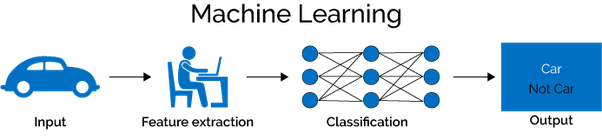
\includegraphics[scale=0.5]{MachineLearningvsDeepLearning.png}
	\caption{Figure showing the process of traditional image classification using feature extraction(Image taken from TowardsDataScience)}
	\label{fig:FeatureExtraction}
\end{figure}


 Computers see images as pixel values, and each image can be viewed as a 2D matrix of pixel values. When building a machine learning pipeline to classify an image, we need to be able to tell what is unique about each image so that the classifier shown in figure~\ref{fig:FeatureExtraction} can correctly classify. This uniqueness in an image can also be viewed as the features. Classification can then be thought of as detection of features in an image, and if features associated with a class are present in the input, we can predict if the input image is of a specific class \cite{MIT.2019}


 In order to build a classification pipeline, the model needs to know what features it is looking for in an input image. These features it is looking for are a predefined set of features. In order to apply this rule, we can leverage human knowledge about a picture in a given domain and extract the most important features. We can then detect those manual features and use that detection to make a classification prediction \cite{popescu2014feature}

 However, images can have lots of variation. If we want to build a robust pipeline, our model needs to be invariant to image variation, while still being sensitive to the differences in individual classifications. Manual features defined by humans can be used, but where this manual detection breaks down is in the detection task itself, and this is merely based on the fact that one class can have incredible amount of variation. This can be illustrated with the ~\ref{fig:FeatureExtractionIssue} provided by \cite{szegedy2015going}
 
 \begin{figure}[H]
 	\centering
 	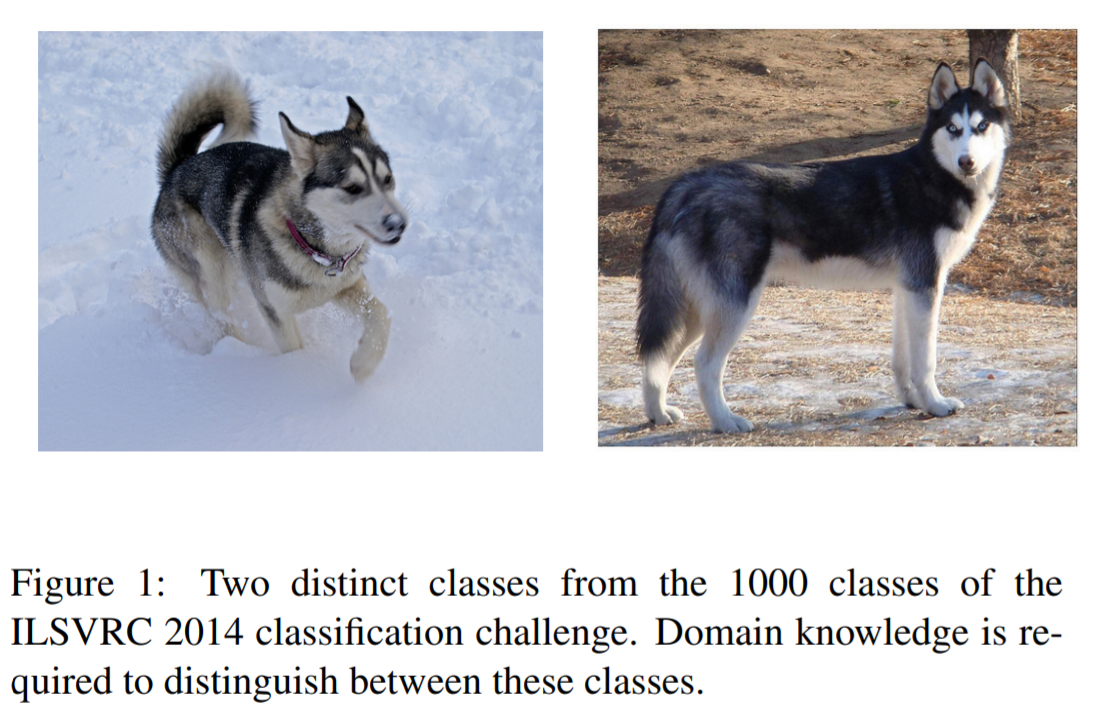
\includegraphics[scale=0.5]{DomainKnowledgeIssueGoogleNet.png}
 	\caption{Two distinct class from 1000 classes of the ImageNet database. Domain knowledge is required to distinguish between separate classes}
 	\label{fig:FeatureExtractionIssue}
 \end{figure}
 

 So, how can we do better? We want a way to both extract features and detect their presence in an image automatically. This is where deep learning can be harnessed to extract features, no matter how the image is presented, automatically.
\section{State-of-the-Art}

Convolutional Neural Networks are a special kind of Multi-layered Perceptron(MLP). Like almost every other neural network they are trained with a version of back-propagation algorithm. Where they differ is in the architecture. This contrast can be viewed in figure~\ref{fig:MLP} and figure~\ref{fig:CNN}. CNN's are designed to recognise visual patterns directly from pixel values with minimal preprocessing. They can recognise patterns with extreme variability(such as handwritten characters) and with robustness to distortions and simple geometric transformations. \cite{lecun1989backpropagation}
CNN's differ from MLP's in that they take advantage of spatial information of an image by convolving a patch of the input image with a filter weight of the same dimension. This results in a 2D matrix called a feature map. These filter weights are applied over the whole image and are iteratively refined in the training process , so that the correct features can be extracted. Different weight filter can be used to extract different features. This is achieved by passing the input across multiple convolution layers. In order to visualise this please refer to figure ~\ref{fig:CNN}. From the diagrams it can be appreciated that MLP's lose all spatial information about an image by flattening every pixel and connecting these pixel values to a neuron in the hidden layer. As well as this we can see that MLP's have many more parameters in the network compared to CNN which can lead to over-fitting especially if the number of training samples is limited. \cite{szegedy2015going}
Starting with LeNet-5 , CNNS's have typically had a standard stacked structured of convolutional layers, followed by ReLU operation, max-pooling and then a fully connected layer. There are variants of this basic design in different image classification tasks and they have all yielded respective results on classification tasks such as MNIST and CIFAR. Although, the most notable includes the ImageNet classification challenge where 1.2 million images were classified into 1000 different classes. In the past years CNN architectures have dominated this challenge and the first publication using CNN architecture was produced by Alex Krizhevsky and Geoffery Hinton in 2012\cite{krizhevsky2012imagenet}. The architecture was given the name Alex-Net and achieved a top-5 error rate of 15.3\% outperforming the previous state-of-the-art, SIFT \cite{lowe2004distinctive} which achieved a 26.2\% error rate using traditional methods. Since then, new CNN architectures have been published with improved results and this can be seen in the table below. 

\begin{figure}[H]
	\centering
	\includegraphics[scale=0.5]{MLP.png}
	\caption{Architecture for MLP. Shows how all pixels value in image are flattened losing all spatial infromation(\url{https://alexlenail.me/NN-SVG/index.html})}
	\label{fig:MLP}
\end{figure}


\begin{figure}[H]
	\centering
	\includegraphics[scale=0.5]{CNN.png}
	\caption{Architecture for Le-Clun CNN. Shows how spatial information is preserved as well different operations applied (\url{https://alexlenail.me/NN-SVG/LeNet.html})}
	\label{fig:CNN}
\end{figure}

\begin{table}[H]
	\centering
	\small
	\begin{tabular}{llll}
		\toprule 	Model & Top-5 error rate &Number of Layers\\
		\midrule
		AlexNet(2012)  & 15.3\%	&  8 layers\\
		VGG16(2014)&7.3\%  & 19 layers\\
		GoogleNet(2014)&6.7\% & 50 layers\\
		InceptionV3(2015)&3.58\%& 50 layers\\
		ResNet(2015)    &3.57\% &152 layers\\
		\bottomrule
	\end{tabular}


	\caption{Results of different models with Human error rate at 5.1\%}\label{tab:Results}
\end{table}




From the table we can see that for large datasets such as ImageNet, there is seems to be a trend developing. That is that the number of layers as well as layer size is increasing. A bigger size means that the model holds more parameters and can make it more prone to over-fitting. To address this problem, a technique developed by Goolge called ``dropout" was developed \cite{hinton2012improving}

\section{Related Work}

Many papers have been published in the domain of using deep learning for medical image analysis. This has been spurred in part due to large carefully curated labelled datasets which have led to papers showing expert-level performance on many medical image classification tasks \cite{irvin2019chexpert}. In this section we will review work related to the thesis title. 


\setcounter{secnumdepth}{4}

\subsection{CheXNet}
In this project, led by Stanford ML Group, an algorithm was developed to interpret chest X-ray images and detect if Pneumonia is present while showing a heat map of the area in the image that had the highest activations \cite{rajpurkar2017chexnet}. Example output can be see in figure~\ref{fig:CheXNetExample}


\begin{figure}[H]
	\centering
	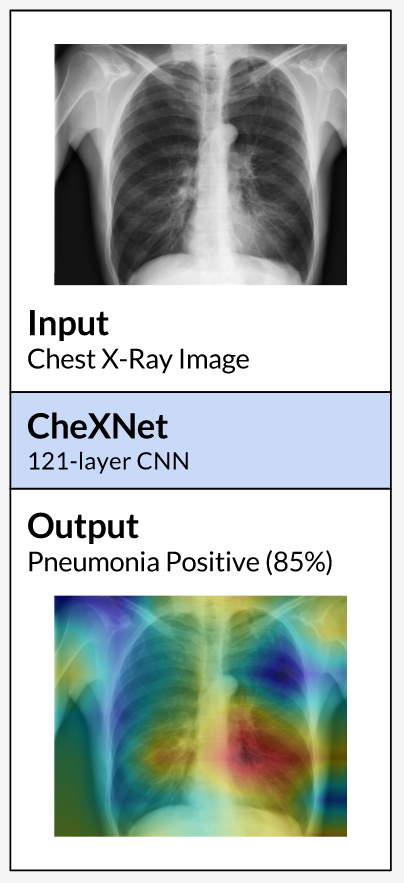
\includegraphics[scale=0.5]{HeatMap.png}
	\caption{Example of CheXNet output of class label along with probability from softmax layer and heat-map}
	\label{fig:CheXNetExample}
\end{figure}

Results showed that the algorithm can detect the pathology at a level exceeding radiologists. The algorithm used a 121-layer CNN which was trained on ChestX-ray14 \cite{wang2017chestx} which is currently the largest publicly available chest X-ray dataset, containing over 100,000 frontal view images and 14 different pathologies. The CNN used is based on the DenseNet architecture \cite{huang2017densely} but modifications were made for single output in the fully connected layer by applying a non-linearity sigmoid function, so that only Pneumonia would have a probability. Pre-trained weights were initialised from a model trained on ImageNet \cite{deng2009imagenet} to speed up the process of training. 
\subsubsection{Results}
Precautions were put in place to make sure that patient images between training and testing sets never overlap. In order to test the accuracy of the model, 420 chest X-rays were collected and 4 practising radiologists annotated where they think the Pneumonia is present. Through the CheXNet tests it showed the algorithm exceeds average radiologist performance on the \textbf{F1 metric}. The model was comparative with expert radiologists on metrics such as \textbf{accuracy}, \textbf{sensitivity} and \textbf{specificity}. The biggest difference was in terms of speed as radiologists took around 4 hours on average to interpret the images whereas CheXNet algorithm took less than 2 minutes \cite{rajpurkar2017chexnet}. Results from figure~\ref{fig:F1Score} present the F1 score for algorithm and average of the 4 clinicians. 

\begin{figure}[H]
	\centering
	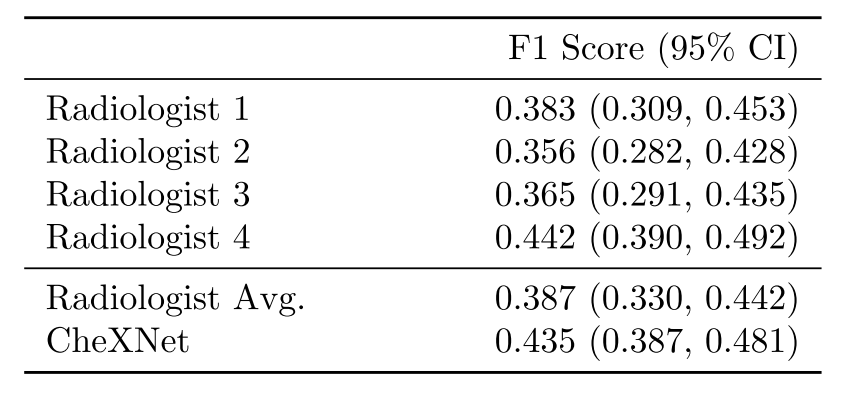
\includegraphics[scale=0.5]{F1Score.png}
	\caption{F1 Score for CheXNet and average F1 score for 4 radiologists}
	\label{fig:F1Score}
\end{figure}
\setcounter{secnumdepth}{4}
\subsection{Multi-task Learning for Chest X-ray Abnormality}
In this paper, researchers built a model trained on 297,541 chest X-rays. The system is based on a novel multi-task deep learning architecture that in addition to classifying and showing a heat-map of the abnormalities also supports the segmentation of the lungs and heart \cite{guendel2019multi}. The research demonstrated that by training the model concurrently on these tasks, one can increase the classification performance. This research produced state of the art performance of 0.883 AUC on average across 12 different abnormalities. ChestX-Ray 14 \cite{wang2017chestx} and PLCO datasets were combined to increase the amount of variability of images and this also showed increase in performance. 

As mentioned before techniques were applied to increase accuracy. One of the methods employed was to normalise the images. A challenge in processing chest radiographs is that there can be large variabilities in the appearance of the image and this is due to the acquisition source, radiation dose \cite{guendel2019multi}. The paper proposes to dynamically window each image by adjusting the brightness and contrast via a linear transformation of the image intensities. Example of output is shown in figure~\ref{fig:Normalisation} 


\begin{figure}[H]
	\centering
	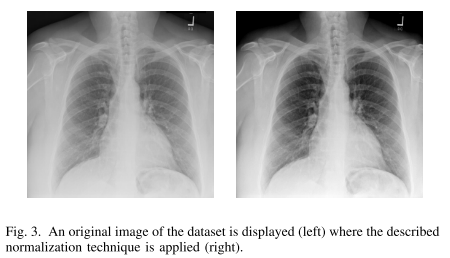
\includegraphics[scale=0.7]{NormalisationTechnique.png}
	\caption{We can see that certain parts of the X-ray become more visible hence making abnormalities more clear for the model}
	\label{fig:Normalisation}
\end{figure}

In addition , the paper also harnesses spatial knowledge related to individual pathologies as well as underlying structure i.e the heart and lungs which can be exploited to increase classification performance. The paper proposes that once can focus the learning task to the heart and lung region as information outside of these regions may be regarded as irrelevant for the diagnosis of heart/lung abnormalities. 

In order to achieve this segmentation, a DenseNet model shown in figure~\ref{fig:DenseNet} \cite{huang2017densely} has been used and figure~\ref{fig:Segmentation}  presents the architecture as well as an example showing the segmentation technique. Another technique that was used to take advantage of spatial information was the use of several approximate spatial labels provided in the PLCO dataset. For five abnormalities(Nodule,Mass,Infiltrate,Atelectasis,Hilar Abnormality) there are rough location information available  to help the model locate where the abnormality is usually located.



\begin{figure}[H]
	\centering
	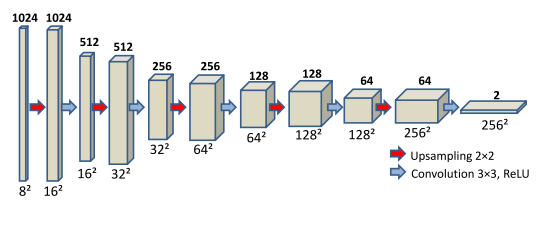
\includegraphics[scale=0.7]{DenseNet_Architecture.png}
	\caption{Architecture for DenseNet}
	\label{fig:DenseNet}
\end{figure}

\begin{figure}[H]
	\centering
	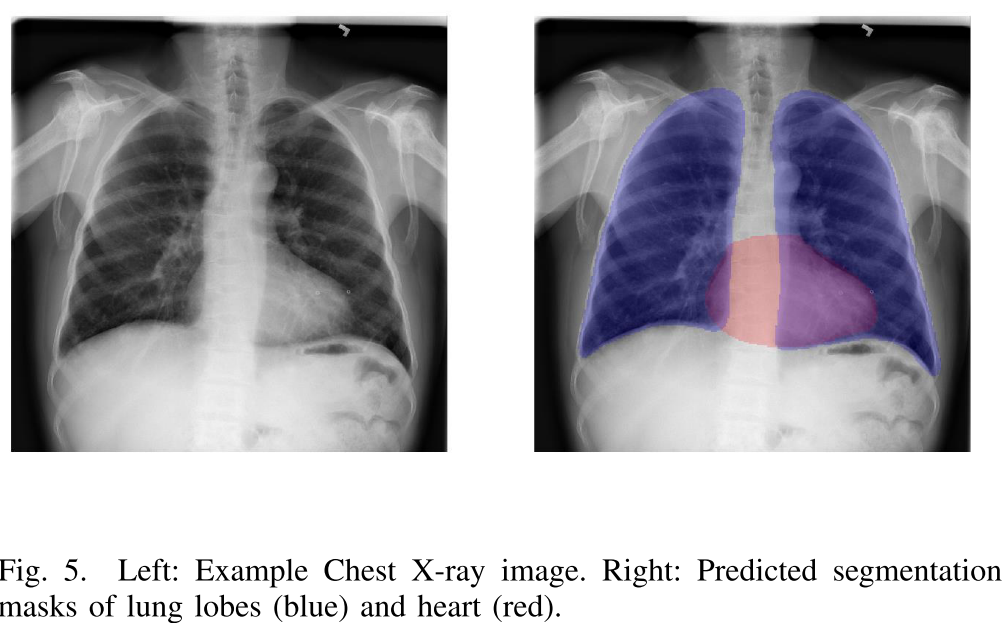
\includegraphics[scale=0.4]{Segmentation.png}
	\caption{Distinct segmentation of lungs and heart}
	\label{fig:Segmentation}
\end{figure}



\subsubsection{Results}


For this paper, different experiments were undertaken to show the performance of the model. As a baseline, performance was measured by only training the classification part on the PLCO dataset. The test was evaluated with an average \textbf{AUC} score across 12 abnormalities of \textbf{0.859}. \par
Results also showed improved classification scores when the network was additionally trained to generate lung and heart segmentation masks (as shown in  figure~\ref{fig:AUC}). Performance increased to 0.866 on average across the abnormalities. \par
As mentioned another technique was to use spatial knowledge and the impact of this showed an average improvement of 0.011\par
This paper also used 2 datasets and by combining both, the average AUC score reaches 0.870. This increase in score is due to more variability in the learning process. As well as this the normalisation technique previously shown in figure~\ref{fig:Normalisation} was applied when training the model and this had a 2 fold benefit. The first was that the training process was reduced on average 2-3 times. The researchers hypothesised that this is due to the images being more aligned in terms of brightness and contrast. Another reason was due to the generalisation of the model parameters and this lead to a performance gain of 0.876. \par
Finally, the researchers upscaled the input image size to 512 in each dimension and adjusted the DenseNet layer to take in 16x16 patch size at each layer. This final network architecture change also added all of the previous techniques mentioned before. The following image shows the results obtained across all techniques and finally the result of combining all the techniques which produces a state-of-the-art performance of \textbf{0.883}



\begin{figure}[H]
	\centering
	\includegraphics[scale=0.4]{AUC_Scores.png}
	\caption{Results showing increasing mean AUC score}
	\label{fig:AUC}
\end{figure}
\setcounter{secnumdepth}{4}
\subsection{Abnormality Detection and Localization in Chest X-Rays using Deep Convolutional Neural Networks}

For this paper, researchers conducted experiments on three datasets. From the datasets, researchers explored the performance of various deep CNN's for detection of heart disease from chest X-rays. Researchers used binary classification on diseases such as Cardiomegaly against normal images \cite{islam2017abnormality}. The paper explores several CNN models such as AlexNet, VGG-Net and ResNet. These models have different layers and typically achieve higher accuracy as layers increase as noted in State-of-the-Art section.

Another part of the research, similar to previous papers reviewed was to produce a heat-map showing which areas of the X-ray the model has the highest activation on. This paper used the sensitivity of softmax scores of occlusion on a certain region in the chest X-ray to find which region in the image is responsible for the classification decision.  
\subsubsection {Results}

The first experiment used single model CNN's on the Indiana dataset, and from the tests, it was shown that deeper models like VGG-19, ResNet improve the accuracy significantly. It was found that Cardiomegaly detection improves 6\% compared to using shallower models like AlexNet. Although results showed high specificity for ResNet-101 and high sensitivity for VGG-16, the VGG-19 gave the highest AUC score of 0.94. This at least 1\% higher AUC for other models. 
As well as this, dropout was used, which increased performance on the shallower networks but degraded deeper ones. For all experiments, it was noted that extracting features from earlier layers lead to improved accuracy of 2-4\%. It was concluded that shallower networks were better for detecting smaller objects, and as an example, it was found that shallower layers from ResNet-15 trained on Cardiomegaly had better performance than later layers across different metrics. figure~\ref{fig:Shallow} shows a more in depth picture of findings. 

\begin{figure}[H]
	\centering
	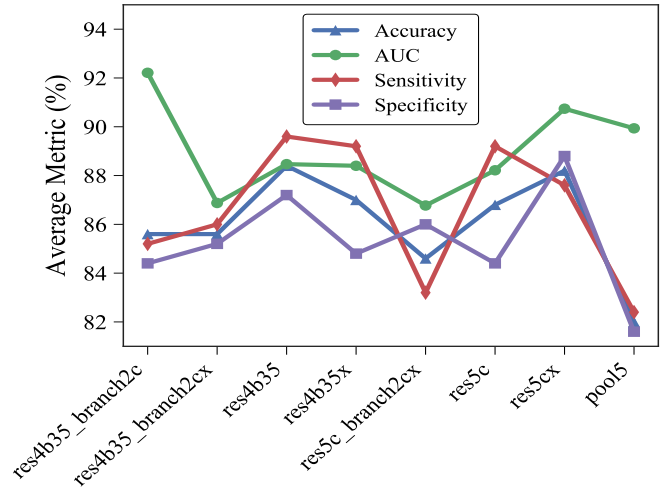
\includegraphics[scale=0.7]{ShallowerLayers.png}
	\caption{Researchers showed that shallower layers in models had a higher accuracy on Cardiomegaly detection compared to deep layers}
	\label{fig:Shallow}
\end{figure}

Another fascinating result was on the localisation of Cardiomegaly shown in the image below. It can be observed that from the figure~\ref{fig:Cardiomegaly}, the model has higher activations from the heart region, which is expected as Cardiomegaly concerns abnormal enlargement of the heart. What was revealing was that other than an enlarged heart for a patient with Cardiomegaly, there is not much difference in features between a normal image and an image classified as Cardiomegaly. But the model can still differentiate between a normal heart which is enlarged due to age or physical attributes of the patient. 
\begin{figure}[H]
	\centering
		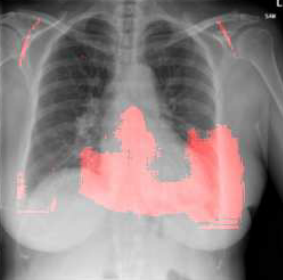
\includegraphics[scale=0.7]{CardiomegalyMap.png}
	\caption{Occlusion sensitivity used to create heap map of region where it thinks Cardiomegaly exists }
	\label{fig:HeatMap}
\end{figure}

\begin{figure}[H]
	\centering
	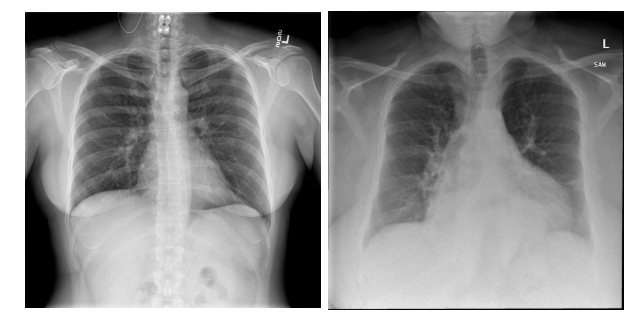
\includegraphics[scale=0.7]{NormalVsCardiomegaly.png}
	\caption{Example of normal heart on the left and Cardiomegaly diagnosed heart on the right }
	\label{fig:Cardiomegaly}
\end{figure}



Finally, another point raised in the paper was the model used for localisation of cardiomegaly were counter-intuitive to traditional methods of cardiomegaly diagnosis, which consider the relative size of heart and lung. But, most of the signals contributing to the softmax score come from the heart alone indicating features in the shape of the heart and its surrounding region alone help in detection of the pathology and perhaps the lung and relative size to the heart are less critical in the diagnosis for the model. 
 

 
 









\include{LiteratureReview/ReviewOfRelatedWork}
\section{Medical Images}

As mentioned in the Overview section, radiology departments in the UK have struggled to meet imaging diagnostic demands. The survey published by the Royal College of Radiology reported 97\% of radiology departments were unable to do so within their working hours. As mentioned in the paper, ``It points to an insufficient number of radiologists to meet the increasing demand for imaging and diagnostic services". According to the report it cited that radiology has the second lowest proportion of trainees to consultants: 26 trainees to every 74 consultants. This is compared to an average in all specialities of 40 trainees for every 60 consultants. The report also cites that there was a particular workforce shortage prominent in Scotland, where the consultant workforce grew by 7\% from 2010 to 2016 but demand for CT,MRI scans increased by 10\%. 
One of the profound impacts of such shortage is the risk to patient care as well as economical effects. The NHS paid nearly £88m in 2016 for backlogs of radiology examinations to cover backlogs of radiology examinations to be reported. To cover these backlogs 92\% of radiology departments paid staff overtime, 78\% outsourced to private companies and 52\% employed ad hoc locums. This amount could have paid for at least 1028 full time radiology consultants.\cite{rimmer2017radiologist}

Given this what has been done to augment the analysis of medical images in the NHS and reduce extreme workload and large expenses ? One particular software which has bee used in the clinical setting is Computer Aided Diagnosis(CAD). CAD is technology which is designed to decrease observational oversights and false negative rates for physicians interpreting medical images such as mammographies \cite{castellino2005computer}. According Dr. Paul Chang, the reason this type of software did not receive as much attention, compared to the possibility of using deep learning, was that it used traditional methods of machine learning. \cite{youtube}

\subsection{Challenges}

There many challenges associated when applying new technologies in a clinical setting. Medical images are very large and complicated and for most of the image classification tasks in the ImageNet example , distinct features or pixels can be learned by a model. Dr. Matthew Lungren , radiologist at Stanford Medical Center, mentioned how most of the pixels in a chest X-Ray from a healthy person who happens to have lunge cancer , will tell you that the image is of a healthy person. But there is only a small proportion of the image which indicates the finding of lung cancer fo the classifier. Dr Lungren also noticed how medical images may have, what is known as artefacts or tokens in the image. Doctors are able to deal with context when looking at an image , but such artefacts or tokens may lead to a model making a decision with higher degree of confidence but in actual fact the classification is incorrect \cite{DrLungren.2018}


\section{Summary of Review}

From the review, it is quite evident that with the ever-growing concern in the NHS of a shortage of radiologists \cite{rimmer2017radiologist}, solutions need to be found in order to solve the issue of increased backlogs. Image classification, as mentioned, can provide augmentation of diagnosis of X-rays. Great leaps and bounds have been made in the field of deep learning and particularly well know CNN architectures show performance exceeding that of human intelligence in the case of ImageNet challenge \cite{krizhevsky2012imagenet}s. As well as this more sophisticated example of applying deep CNN's to medical images has shown outstanding results on pathologies such as Pneumonia and Cardiomegaly \cite{rajpurkar2017chexnet}. This problem of diagnosing X-rays also comes with its challenges which have been outlined in the challenges section. Other hurdles must be kept in mind for implementation purposes, and these include making sure that pixel values are not lost. Given the nature of X-rays, pixel loss can lead to pathologies being removed from an image such as lung nodules and according to the Royal  College of Radiologists certain rules needs to be adhered to so that images do not lose quality when it comes to diagnosing them. Lastly, when training a model on medical images, the dataset chosen needs to be balanced in class labels. As well as this one of the big obstacles is lack of datasets of reliable labelling of datasets as noise in class labels can lead to reduced performance. 


\section{Conclusion}

In this section, we will conclude how the rest of this thesis will be implemented and how the proposed problem in the introduction will be approached. From the findings above the aim is to apply one of the well known CNN architectures to build an accurate image classification pipeline on predicting the presence of Pneumonia in chest X-rays. In order to train the model, a carefully curated dataset must be chosen.  The dataset that will be used in this thesis comes from a public dataset carefully curated by Stanford ML Group called CheXPert. This dataset was created to solve three problems which include enough instances, strong reference standards and provide human performance metrics for comparison. It consists of 224,316 chest X-rays, and one of the main obstacles in the development of these datasets is the lack of strong radiologist-annotated ground truth.
The objectives is to build an accurate model which can predict and localise the Pneumonia with techniques such as occlusion. Another objective would be to build an interface which allows the entry of a chest X-ray and a predicted class label will be given back as well as a heat-map indicating which parts of the image had the highest activation. 
Lastly, if results from the initial pipeline show high accuracy, specificity, sensitivity and AUC, then the model could be extended to classify more than one pathology contained in the dataset.


\include{RequirementsAnalysis/RequirementsAnalysis}




\chapter{Experiment Setup}

Before moving onto explaining process of applying the machine learning models for this paper, the following chapters explains the experimental setup that took place before starting the experiments. In this section the hardware and software setup is discussed. As well as this a general overview of the dataset that is used for the experiments is discussed and more importantly the preprocessing that had to occur before running experiments is explained. Lastly evaluation metrics will be discussed so that experiments in the later chapters can be analysed against metrics that determine the success or failure of an experiment

\section{Hardware Implementation}

A computer system with the specifications shown in Table \ref{fig:DGX} will be used to carry out the experiments in this paper. Through the help of Robert Gordon University's Research Hub for Artificial Intelligence, this project makes use of the Research Hub's Nvidia DGX-1 to accelerate the deep learning experiments carried out in this paper. 

\begin{table}[H]
	\centering
	\small
	\caption{Computer System Specification}
	\label{fig:DGX}
	\begin{tabular}{ll}
		
		\hline
		Operating System & Ubuntu 18.04 Linux Host OS\\
		
		\hline
		CPU & 2x Intel Xeon E5-2698 v3 (16 core, Haswell-EP) \\
		\hline
		System Memory & 512GB DDR4-2133 (LRDIMM)\\
		\hline
		GPU & 8x NVIDIA Tesla P100 (3584 CUDA Cores)\\
		\hline
		GPU Memory & 128GB HBM2 (8x 16GB) \\
		\hline
	\end{tabular}
\end{table}


\section{Software Implementation}

The setup for the experiments in this paper involves the use of \textbf{Python 3}. The solution heavily relies on \textbf{Keras}, which is an open-source neural network library written in python and is capable of running on top of \textbf{TensorFlow} as its back-end. Keras is designed to enable fast experimentation with deep neural networks and contains the basic building blocks to build one such as adding layers, objective functions, activation functions and optimisers. Moreover, Keras through the use of TensorFlow allows for the use of distributed training of deep learning models on multiple Graphics Processing Units - GPUs. This is further achieved by using CUDA, which is a parallel computing platform and Application Programming Interface(API) created by Nvidia. 
The CUDA platform is a software layer that gives direct access to the GPU allowing for highly parallel manipulation of large blocks of data.




\section{Dataset}


The dataset that will be used for training and testing of the learning algorithm has been taken from a public repository \cite{Dataset}. The dataset includes X-ray images of both normal patients and patients with pneumonia infected lungs. Based on the information given by the authors that published the dataset, for use in the paper titled ``Identifying Medical Diagnoses and Treatable Diseases by Image-Based Deep Learning"  \cite{kermany2018identifying}, the data has been obtained from the Chest X-ray images selected from a respective cohort of pediatric patients aged from one to five years old from Guangzhou Women and Children's Medical Center. 

The dataset comes with two folders which include training and validation. Each folder contains subfolders for each type of classification, normal and pneumonia. The training folder contains 5218 images split into 1342 normal images and 3876 pneumonia images. The validation folder contains 624 images split into 234 normal images and 390 pneumonia images.
Figures \ref{fig:TrainingDist} and \ref{fig:TestingDist} help to visualise the distribution of the training and testing set respectively. The distribution of both training and testing are important to notice as this will be an important consideration when evaluating the model performance. 

  \begin{figure}[H]
 	\centering
 	\includegraphics[scale=0.7]{images/TrainingSet_dist.png}
 	\caption{Class Distribution of Training Set}
 	\label{fig:TrainingDist}
 \end{figure}
 
 \begin{figure}[H]
 	\centering
 	\includegraphics[scale=0.7]{images/TestingSet_dist.png}
 	\caption{Class Distribution of Testing Set }
 	\label{fig:TestingDist}
 \end{figure}

To visualise the images used to train the learning algorithm, figure \ref{fig:normalX-ray} and \ref{fig:pneumoniaX-ray} shows an example of both a normal patient and a patient suffering from pneumonia. It might be noticeable in figure \ref{fig:normalX-ray} that a healthy X-ray would normally be clearer, and the general area of the chest is more visible compared to cases where pneumonia is present, as shown in figure \ref{fig:pneumoniaX-ray}. However, the onset of pneumonia in patients can differ depending on the severity of the infection. As such, there may only be a few pixels that denote the presence of pneumonia which makes the task of detecting the disease a challenge. 

 \begin{figure}[H]
	\centering
	\includegraphics[scale=0.1]{images/normal.jpeg}
	\caption{Normal Chest X-ray}
	\label{fig:normalX-ray}
\end{figure}

\begin{figure}[H]
	\centering
	\includegraphics[scale=0.1]{images/pneumonia.jpeg}
	\caption{Pneumonia Chest X-ray}
	\label{fig:pneumoniaX-ray}
\end{figure}







\subsection{Dataset Preprocessing}
% Oh hello there, here are some tasks: 
% 1. Remove 'due to the fact' on line 5 - its a filler-word
% 2. Change due to guidance on line 5

During exploration of the dataset it was shown that the X-ray images provided were of different sizes. This most likely due to different X-ray imaging machines used during collection of the dataset. Before applying the learning algorithm on the X-ray images we needed to make sure that each input image was of the same dimension. This is due to the way a CNN is configured via libraries like Keras, where the size of the input layer is constant. At first, all images were resized from their original size to 250 x 250. However, due to guidance, later experiments used a size of 256 x 256. 



\subsection{Normalising Images}

Data normalisation is an important step which ensures each pixel value for an image has a similar data distribution. This makes convergence faster while training a neural network. Although non-normalised data can be presented to the neural network, this can result in challenges during training, such as slower training of the model. 

As discussed in section \ref{sect:SotA}  ``State of the Art" , neural networks process inputs using small weight values which are multiplied by the input value. If these inputs are on a large unsigned integer scale, like pixel values, this may disrupt or slow down convergence of the training process. A pixel value of 0(white) compared to 255(black) are both equally as important but the 255 value will have a greater effect on the final prediction. This large value could cause the output to be wrong and lead to the training process taking longer. 

For the purposes of this paper, data normalisation is applied by dividing each pixel value by 255 and as a result all inputs to the model have a range between 0 and 1.

To better understand the stages of normalisation, figure \ref{fig:preprocessing} shows the steps taken to normalise each image.
\footnote[1]{\href{https://github.com/jozi98/HonoursProject/blob/master/ChestX-ray.ipynb}{Python Notebook:Preprocessing }} 

 \begin{figure}[H]
	\centering
	\includegraphics[scale=0.2]{images/Preprocessing.png}
	\caption{Stages of the Preprocessing and Normalisation}
	\label{fig:preprocessing}
\end{figure}


 


\section{Going Beyond Accuracy}\label{metrics}


As shown in figure \ref{fig:TestingDist}, the class distribution of the testing set is imbalanced. Due to this imbalance, it is important to look beyond accuracy to validate a model performance. For example, since the test set is imbalanced, if all the test cases were labelled positive, i.e. a class label of pneumonia, then the accuracy on the test set would be 63\%. However, the accuracy does not show the underlying performance of the model, which indicates that it is classifying every patient as having the infection.


Due to the domain of this paper and its aim: Automatic classification of X-ray Images as either normal or abnormal, a confusion matrix needs to be considered when evaluating results. Figure \ref{fig:ConfMatrix} shows an example of a confusion matrix that will be used to analyse results. The number of pathological samples that are \textit{correctly} identified as a pathological sample by the model is called a true positive (TP). The number of pathological samples that are \textit{incorrectly} classified as normal by the model is called a false negative(FN). The number of normal samples that are \textit{correctly} identified as normal is called a true negative(TN) and in a similar fashion, the number of normal samples that are \textit{incorrectly} identified as pathological samples is called false positive(FP). 
Given the domain of this study, the cost of a false negative is higher than a false positive

	
 \begin{figure}[H]
	\centering
	\hspace{-2cm}
	\includegraphics[scale=0.6]{images/ConfusionMatrix}
	\caption{Confusion Matrix}
	\label{fig:ConfMatrix}
\end{figure}



Although accuracy is still considered, this study will also examine the values of precision, recall/sensitivity and specificity. Accuracy, specificity, recall and precision are computed as follows:

\begin{center}

\[Accuracy=\frac{TN+TP}{TN+FP+FN+TP}\]
\vspace{.5em}
\[Specificity=\frac{TN}{TN+FP}\]
\vspace{.5em}
\[Recall/Sensitivity=\frac{TP}{TP+FN}\]
\vspace{.5em}
\[Precision=\frac{TP}{TP+FP}\]
\end{center}







\begin{itemize}
	
	\item \textbf{Accuracy} is a basic measure shown as a percentage of the total correct classification out of all the samples in the testing set.
	\item \textbf{Specificity} shows the degree to which the model correctly identifies normal samples as normal. 
	\item \textbf{Recall/Sensitivity} is a measure which shows the degree to which the model does not miss a pathological sample
	\item \textbf{Precision} is measure of the exactness or quality of the model when it returns results for a specific class
	
	
\end{itemize}






\renewcommand{\clearpage}{}

\chapter{Experiment \& Results}


In this chapter, the experiments that were performed during the duration of this project will be discussed. This discussion will include the successful experiments as well as the experiments that failed due to a flaw in the initial setup. For each experiment the general setup will be discussed. This includes the CNN architecture, epochs, batch size, learning rate and training and testing splits. Each of the experiment results will be discussed in detail where the evaluation metrics from \ref{metrics} will be applied to the model results.  

\section{Experiment 1}



\textbf{Model Architecture:} 
For the first experiment that was carried a simple CNN architecture was used to classify the images. The setup of the CNN involved the use of two convolutional layers each with ReLU activation. After the final convolutional layer, Max Pooling is applied to reduce the dimensionality of the network. After applying Max Pooling the features extracted are flattened and sent through a fully connected layer consisting of 128 neurons. ReLU activation is applied once more before adding a further 2 neurons and finally a Soft-max layer. Figure \ref{fig:exp1} shows the layers that have been used in Experiment 1


\begin{figure}[H]
	\centering
	\includegraphics[scale=1,width=1\linewidth]{images/Experiment1_Architecture}
	\caption{Model Architecture for Experiment 1}
	\label{fig:exp1}
\end{figure}



\textbf{Hyper-parameters}

Hyper-parameter setup for the experiment is the following: 

\begin{itemize}

\item Imbalanced training set(\textit{Non-Shuffled})
\item Balanced testing set 
\item Batch Size = 64
\item Epochs = 1
\item Adam optimiser (lr=0.01) 
\item Categorical Cross Entropy Loss Function


\end{itemize}

\textbf{Results}

For the initial experiment, the following confusion matrix shows the models performance: 

 \begin{figure}[H]
	\centering
	\hspace{-3cm}
	\includegraphics[scale=0.5]{images/ConfusionMatrix_Exp1}
	\caption{Experiment 1 Confusion Matrix}
	\label{fig:exp1_conf}

\end{figure}
\newpage

After inspecting the results above, it can be observed that the model trained on the above hyper-parameters has an accuracy of 50\%  on the test set shown in the confusion matrix above. From the matrix, it shows the model has a Recall/Specificity score of 1 since the model was able to identify all patients with pneumonia. However, although the model can classify pneumonia cases correctly, the opposite is true for the normal cases as the model classifies them as positive cases, hence giving a Specificity score of 0.


Observations were made to understand why the model produced the results in figure \ref{fig:exp1_conf}. Upon reviewing the setup for experiment 1, it was noted that since the training data was not shuffled it meant that for each epoch the model was learning 74\% of the pneumonia cases first and a further 26\% of the normal cases. It meant that the model was learning in a sequential manner which affects the weight updates. It is important that moving forward the training set is shuffled so that batches of input contain a mixture of both positive and negative samples. 

Another observation noted when reviewing results is that the number of epochs was too low. The number of epochs determines the number of passes over the entire training set. It means the number of epochs must be higher so that the model has more chances to learn from the training set.


Lastly, in this experiment, it was decided that the testing should be balanced. However, after reflection experiments going forward should not balance out the testing set as this could remove vital images which could include difficult samples and may test the model's capability further. Balancing of the provided data would not reflect the medical environment where it is common to have imbalanced datasets. 
 
 
\newpage
\subsection{Improving Experiment 1} \label{Improving Experiment1}

\textbf{Model Architecture}
In this experiment, the aim is to see the effect higher epochs and shuffled training data has on the model performance.
The model architecture is the same as the previous experiment which is illustrated in figure \ref{fig:exp1}. 

\textbf{Hyper-parameters}

\begin{itemize}
	
	\item Imbalanced training set(\textit{Shuffled per epoch})
	\item Validation set(\textit{10\% of training})
	\item Imbalanced testing set 
	\item Batch Size = 64
	\item Epochs = 10
	\item Adam optimiser (lr=0.01) 
	\item Categorical Cross Entropy Loss Function
	
\end{itemize}

The main differences in hyper-parameters settings include increased epoch to allow the model to have more passes to learn from the training data. The training set has also been shuffled and the testing set has been changed to the unbalanced distribution mentioned in the previous experiment. To track the model performance over the entire training process this experiment used 10\% of the training set to act as a validation set. By doing so we can track the model accuracy and loss over 10 epochs. 

\textbf{Note:} Keras allows us to shuffle the data via the \textit{shuffle} parameter which shuffles the order of the data at every epoch. This allows the model to learn in a varied manner since the sequence of the training data is different per epoch. By using this feature in Keras it means reproducibility is not guaranteed but experiments ran multiple times should show similar results. 

\textbf{Results}

For this experiment, the following confusion matrix shows the model performance after changing hyper-parameters. Since the model has been run for more than one epoch, an accuracy and loss graph can be used to track the model performance on the training and validation set through out the training process.

\begin{figure}[H]
	\centering
	\hspace{-1cm}
	\includegraphics[scale=0.5,width=0.5\linewidth]{images/CMExp_1_1}
	\caption{Experiment 1.1 Confusion Matrix}
	\label{fig:exp1.1_conf}
\end{figure}




\begin{figure}[H]
	\begin{minipage}[t]{7.2cm}
		\begin{center}
			\includegraphics*[width=1\linewidth]{images/444ff3fd-daba-478a-9d6f-8c8062ddb5b2}
			\caption{Model Accuracy}
			\label{fig:exp1.1_auc}
		\end{center}
	\end{minipage}
	\hfill
	\begin{minipage}[t]{7.2cm}
		\begin{center}
			\includegraphics*[width=1\linewidth]{images/e6bf7a6f-ab58-4092-ab68-5573f8142896}
			\caption{Model Loss}
			\label{fig:exp1.1_loss}
		\end{center}
	\end{minipage}
\end{figure}


\textbf{Results Analysis}


The confusion matrix in figure \ref{fig:exp1.1_conf} shows that after shuffling the training data and increasing the number of epochs the model achieves a 75\% \textbf{Accuracy} on the test set. \textbf{Recall/Sensitivity} score is 0.99 and the \textbf{Specificity} score is 0.3. From figure \ref{fig:exp1.1_auc} we can track the model accuracy on both the training and testing set. The graph shows us the model is able to quickly learn the training set close to 100\% accuracy between the first and third epoch(Python epoch begins from 0th epoch) and continues to increase which suggests the model could have been trained for longer. Figure \ref{fig:exp1.1_loss} shows a similar story but measures the models loss which shows the training loss drops quickly in the first 2 epochs. The validation line in figure \ref{fig:exp1.1_auc} shows the accuracy increases a lot between the first and second epoch, however, later on in the training process validation accuracy tends to fluctuate before it starts to drop. 


Although the model has a reduced Recall/Specificity score, which is expected since the model has learned in a varied manner, the number of false positives has gone down which suggests increased epochs and a shuffled training set improves model performance. However, it still evident that due to the imbalance in the training set the model is classifying almost double the amount of false positives compared to true negatives. To diagnose the issue of why the validation data is suffering from a case of over-fitting the same experiment was ran for four additional runs where the test accuracy ranged from 71\% to 75\%. 

\begin{figure}[H]
	\centering
	\includegraphics[width=1\linewidth]{images/ImprovingExp1_Enhanced}
	\caption{Identical experiments with different outcomes }
	\label{fig:exp1.1_4models}
\end{figure}


Figure \ref{fig:exp1.1_4models} shows that the same experiment ran multiple times results in a different training process, where even though training accuracy for all five experiments ends in a similar trajectory, the validation accuracy shows a different story as all five validation accuracies are different. On reflection the reason the same model produced different accuracies is due to the value of the learning rate being too high for this dataset. 


The learning rate is a hyper-parameter that controls how much to change the model in response to the estimated error each time the model weights are updated. In this specific situation we hypothesis that since the data is shuffled each of the experiments sees a different sequence of data which when coupled with a high learning rate causes drastic changes in weight updates which effects the training and validation accuracy.
















\section{Hyper-Parameter Tuning}

In this experiment(s) the aim is to apply hyper-parameter tuning to improve performance of the previous experiment and stabilise the training and validation accuracy and loss. There are a range of hyper-parameters to experiment with however, the experiments carried out in this section will focus mainly on adjusting Adam learning rate, increasing epochs, changing the number of convolution operations in the convolutional layers and number of dense connections in the fully connected layers.

\subsection{Learning rate}

It was noted in the experiments carried out in section \ref{Improving Experiment1} that after running the same experiment five times the overall testing accuracy varied as well as the validation accuracy and loss. The aim of this experiment is to reduce the learning rate to see the effect it has on stabilising results. 

\textbf{Model architecture}

The model architecture is the same as before and is illustrated in figure \ref{fig:exp1}

\textbf{Hyper-Parameters}

The model hyper-parameters are largely the same with learning rate changing from 0.01 to 0.0001. 

\textbf{Results}

\begin{figure}[H]
	\centering
	\hspace{-1cm}
	\includegraphics[scale=0.5,width=0.5\linewidth]{images/ConfusionMatrix_Hyper_Param(LR)}

	\caption{Confusion Matrix after adjusting learning rate}
	\label{fig:exp1.2LR}
\end{figure}


\begin{figure}[H]
	\centering
	\includegraphics[scale=1,width=1\linewidth]{images/LearningRate_Auc}
	\caption{Model accuracy after changing learning rate}
	\label{fig:exp1.2LRAuc}
\end{figure}

\begin{figure}[H]
	\centering
	\includegraphics[scale=1,width=1\linewidth]{images/LearningRate_Loss}
	\caption{Model loss after changing learning rate}
	\label{fig:exp1.2LRLoss}
\end{figure}

In this particular experiment, although we see a decrease in performance, the same model ran five times produces results clustered closer together with testing accuracy across five models being the same except one which differs by one percent. In figure \ref{fig:exp1.2LRAuc} and \ref{fig:exp1.2LRLoss} we see that for the five models ran, all of them show a similar trajectory with both training and validation accuracy closely follow each other. A change in learning rate also appears to reduce the discrepancy between the training and validation accuracy acting as a regularisation effect which stopped over-fitting. The same can be said for the loss graph show in figure \ref{fig:exp1.2LRLoss} which shows the training loss is still lowering with the validation loss starting to flatten out. This suggests that the model could have been trained for longer. 

Comparing figure \ref{fig:exp1.1_4models} and \ref{fig:exp1.2LRAuc}, we can see that the model after tuning the learning rate is stable across multiple runs. As a result of reducing the learning rate, although it stabilised results, the model has smaller weight updates which slows down the process of convergence. 

Therefore, we ran the same experiment with 20 epochs which resulted in test results shown in the confusion matrix in figure \ref{fig:exp_HyperParam_20epochs_CM} and the model accuracy loss shown in figure \ref{fig:exp_HyperParam_20epochs_ModelAccuracy}  and \ref{fig:exp_HyperParam_20epochs_ModelLoss} respectively. 

\begin{figure}[H]
	\centering
	\hspace{-1cm}
	\includegraphics[scale=0.5,width=0.5\linewidth]{images/Hyper-Param_Tuning/ConfusionMatrix}
	\caption{Results after 20 epochs}
	\label{fig:exp_HyperParam_20epochs_CM}
\end{figure}

\begin{figure}[H]
	\begin{minipage}[t]{7.2cm}
		\begin{center}
			\includegraphics*[width=1\linewidth]{images/Hyper-Param_Tuning/Model_Accuracy}
			\caption{Model Accuracy}
			\label{fig:exp_HyperParam_20epochs_ModelAccuracy}
		\end{center}
	\end{minipage}
	\hfill
	\begin{minipage}[t]{7.2cm}
		\begin{center}
			\includegraphics*[width=1\linewidth]{images/Hyper-Param_Tuning/Model_Loss}
			\caption{Model Loss}
			\label{fig:exp_HyperParam_20epochs_ModelLoss}
		\end{center}
	\end{minipage}
\end{figure}

After running the experiment over 20 epochs, the overall testing \textbf{Accuracy} is 76\% with a \textbf{Recall} and \textbf{Specificity} score of 0.99 and 0.37, respectively. From the model accuracy graph shown in figure \ref{fig:exp_HyperParam_20epochs_ModelAccuracy}, the training process is generally stable when comparing both the training and validation lines, which suggests that a reduced learning rate and increased epoch value has kept stability during training. There are slight deviations after the 9th epoch until the 20th where the training and validation accuracy and loss start to deviate from each other. When comparing the result from the experiment in section \ref{Improving Experiment1}, the results in this experiment after reducing the learning rate and increasing epochs shows a slight increase in \textbf{Accuracy} and \textbf{Specificity}. 



\subsection{Adding Convolution and Fully Connected Layers}

Previous experiments showed that we were able to stabilise results over many runs and increase specificity. Another approach that we took to further reduce the higher number of false positives, is to alter the convolutional and fully connected layer in the model architecture. Figure \ref{fig:exp1_example} and \ref{fig:IncConvo} shows a comparison of the model architecture between the previous experiments and the one used in this experiment. 

\begin{figure}[H]
	\centering
	\includegraphics[scale=1,width=1\linewidth]{images/Experiment1_Architecture}
	\caption{Model Architecture for previous experiments}
	\label{fig:exp1_example}
\end{figure}

\begin{figure}[H]
	\centering
	\includegraphics[scale=1,width=1\linewidth]{images/Experiment_Architecture}
	\caption{New Model architecture}
	\label{fig:IncConvo}
\end{figure}



What is noticeable is the addition of a convolution layer and the number filters in each of those layers. These layers are responsible for extracting the relevant features of an image, before passing those features through a fully connected(FC) layer, where the classification process occurs. Previous experiments maintained the same number of filters in the two convolutional layers, whereas in this experiment we doubled the amount of filters after every layer. The intuition behind this choice is that CNN's typically detect lower level features via the filters from the first convolutional layer, such as edges and lines. Once the lower level features are extracted, the second layer typically detects motifs by spotting particular arrangements of edges, regardless of small variations and finally the third layer may assemble motifs into larger combinations that correspond to parts of familiar objects \cite{lecun2015deep}. By increasing the number of filters, a higher number of inputs are passed to the FC layer, and as such, it makes sense to increase the number of neurons in the FC layer which is why an additional layer of 64 neurons is added. 

Moreover, the addition of Max Pooling helps with reducing the dimensionality of the network after every convolutional operation and lastly, a technique know as dropout was also used in this experiment to help combat over-fitting. Previous experiments showed signs of over-fitting towards the end of the training process and so increasing the number of convolutional layers could increase over-fitting and hence drop performance on the test set. Dropout is a regularisation technique where randomly selected neurons are ignored during training, which means that their contribution to the activation of downstream neurons is temporarily stopped during the forward propagation, and subsequently any weight updates during the back-propagation stage are not applied. Figure \ref{fig:Dropout} shows an example of how dropout works.

\begin{figure}[H]
	\centering
	\includegraphics[scale=0.5,width=1\linewidth]{images/IncConvoLayers/Dropout}
	\caption{}
	\label{fig:Dropout}
\end{figure}

In the paper which introduced the concept of dropout \cite{srivastava2014dropout}, the recommended value for randomly dropping out neurons is 0.5, however for this experiment we will use a value of 0.1 since the FC layer is much smaller in this experiment compared to the original paper and the previous experiments did not show a huge deviation between the training and validation lines.

\textbf{Model Architecture}

As mentioned above the model architecture is shown in figure \ref{fig:IncConvo}. 

\textbf{Hyper-Parameters}

The model hyper-parameters are unchanged from the previous experiment. 

\textbf{Results}

\begin{figure}[H]
	\centering
	\hspace{-1cm}
	\includegraphics[scale=0.5,width=0.5\linewidth]{images/IncConvoLayers/ConfusionMatrix}
	\caption{Testing results after adjusting architecture}
	\label{fig:exp_IncConvo}
\end{figure}

\begin{figure}[H]
	\begin{minipage}[t]{7.2cm}
		\begin{center}
			\includegraphics*[width=1\linewidth]{images/IncConvoLayers/Model_Accuracy}
			\caption{Model Accuracy}
			\label{fig:exp_IncConvo_ModelAccuracy}
		\end{center}
	\end{minipage}
	\hfill
	\begin{minipage}[t]{7.2cm}
		\begin{center}
			\includegraphics*[width=1\linewidth]{images/IncConvoLayers/Model_Loss}
			\caption{Model Loss}
			\label{fig:exp_IncConvo_ModelLoss}
		\end{center}
	\end{minipage}
\end{figure}

Figure \ref{fig:exp_IncConvo} shows the results when testing the trained model on the test set. The results show a small increase in \textbf{accuracy} from the previous experiment of 76\% to 77\%. Although its a small increase, results do show that \textbf{specificity} has increased from 0.37 to 0.41, hence an improvement in the number of true negatives and reduction in false positives. \textbf{Recall} remains high, but this is due to the class imbalance which favours the positive class. The model accuracy and loss for this experiment shows that the training and validation lines are stable during the training process and does not show signs of over-fitting. 










\footnotesize  %NOTE: reduced the size of the text for the bibliography
%NOTE: set the style for the bibliography and display the references used within the document

\bibliographystyle{apacite}
\bibliography{BibTex/References}


\normalsize

\end{document} %NOTE: END of document, nothing after this point
